\documentclass[a4paper,11pt,titlepage]{article}
\usepackage[utf8]{inputenc}
\usepackage{lmodern} \usepackage[T1]{fontenc}
\usepackage[babel=true]{microtype}
\usepackage[portuguese]{babel}
\usepackage[pdftex]{hyperref}
\usepackage{graphicx}
\usepackage{eurosym}
\usepackage{scrextend}
\usepackage{hyphenat}
\usepackage{url}
\usepackage{hyperref}
\usepackage{listings}
\usepackage{indentfirst}
\usepackage{float}
\usepackage[usenames,dvipsnames,svgnames,table]{xcolor}

\lstdefinestyle{customc}{
  belowcaptionskip=1\baselineskip,
  breaklines=true,
  xleftmargin=\parindent,
  language=C,
  showstringspaces=false,
  tabsize=2,
  basicstyle=\footnotesize\ttfamily,
  keywordstyle=\bfseries\color{blue},
  commentstyle=\itshape\color{gray},
  identifierstyle=\color{black},
  stringstyle=\color{OliveGreen},
}

\lstdefinestyle{customcwithlines}{
  belowcaptionskip=1\baselineskip,
  breaklines=true,
  xleftmargin=\parindent,
  language=C,
  showstringspaces=false,
  numbers=left,
  tabsize=2,
  basicstyle=\footnotesize\ttfamily,
  keywordstyle=\bfseries\color{blue},
  commentstyle=\itshape\color{gray},
  identifierstyle=\color{black},
  stringstyle=\color{OliveGreen},
}

\title{\huge \textbf{Aplicação de download e configuração e estudo uma rede\\[1cm] \Large Relatório\\[0.7cm]

\includegraphics{res/logo.png}\\[0.7cm] \large Redes de Computadores\\[0.25cm] \small $3^o$ ano\\[0.05cm]Mestrado Integrado em Engenharia Informática e
Computação\\[1cm]}\normalsize Turma 4}

\author{Carolina Moreira\\Daniel Fazeres\\José Peixoto \and 201303494\\201502846\\200603103 \and  up201303494@fe.up.pt\\up201502846@fe.up.pt\\ei12134@fe.up.pt}

\begin{document}
\maketitle

\newpage
\tableofcontents
\newpage

\abstract
\iffalse dois parágrafos: um sobre o contexto do trabalho; outro sobre as
principais conclusões do relatório \fi

No âmbito da unidade curricular de Redes de Computadores, foi-nos proposto o
desenvolvimento de uma aplicação que testasse um protocolo de ligação de dados
criado de raiz, transferindo um ficheiro recorrendo à porta de série $RS-232$.
O trabalho permitiu praticar conceitos teóricos no desenho de um protocolo de
ligação de dados como o sincronismo e delimitação de tramas, controlo de erros,
controlo de fluxo recurso a mecanismos de transparência de dados na transmissão
assíncrona.

Findo o projeto, notou-se a importância dos mecanismos que asseguram tolerância
a falhas fornecidos pela camada de ligação de dados, uma vez que a camada
física não é realmente fiável.

\section{Introdução}
\iffalse(indicação dos objectivos do trabalho e do relatório; descrição da
lógica do relatório com indicações sobre o tipo de informação que poderá ser
encontrada em cada uma secções seguintes) \fi
O objetivo do trabalho realizado nas aulas laboratoriais da disciplina de Redes
de Computadores é a implementação de um protocolo de ligação de dados que
permita praticar conhecimentos acerca de transmissões de dados entre
computadores, programando em baixo nível as características comuns a este tipos
de protocolos como a transparência na transmissão de dados de forma assíncrona
e organização da informação sob a forma de tramas.

\section{Equipamento: Switch Cisco}

\section{Equipamento: Router Cisco}

\section{Experiência 1: Configuração de uma rede IP }

Nesta experiência, configuraremos apenas uma rede simples de dois computadores
ligados entre si por um switch. Esta rede usará o conjunto de protocolos que
constituem, em parte, a arquitectura da mais conhecida rede de todas, a
Internet. Como é sabido, o protocolo que gere a camada de rede da Internet é
o IP (Internet Protocol).  Para além do próprio protocolo IP, a Internet usa
vários outros protocolos auxiliares para regular o seu funcionamento,
nomeadamente ARP, ICMP, e DHCP.
O protocolo DHCP é usado para negociar automaticamente a atribuição de um
endereço IP a qualquer elemento de uma rede que permita uma identificação única
perante outros membros. Este protocolo não será usado, e em vez disso
atribuir-se-á manualmente e estaticamente endereços IP a cada um dos
computadores das redes desta e subsequente experiências deste trabalho, o que é
exequível visto tratarem-se de redes de pequena dimensão, o que não seria o
caso noutras instalações de aplicação prática no mundo real.

Os endereços desta experiência serão divididos, como é feito neste protocolo de
rede, numa parte respeitante à subrede (subnet), e outra que indicará o
endereço de cada computador dentro desta rede. Um pequeno esquema do resultado
pretendido é indicado na próxima imagem.

\begin{figure}[H]
    \center
    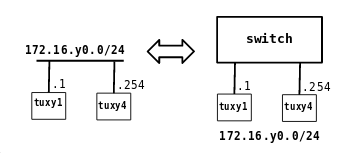
\includegraphics[scale=0.45]{res/network1.png}
    \caption{Rede da 1a Experiência}
    \label{fig:network1.png}
\end{figure}

\subsection{Configuração de interfaces}

Na configuração desta rede, começamos por ligar apenas os computadores TUX1 e
TUX4 ao switch Cisco Catalyst 3560. Cada um dos computadores tem duas
interfaces expostas, para além da loopback.
A interface loopback é uma interface apresentada pelo sistema operativo como
qualquer outra interface, mas possuíndo o endereço especial $127.0.0.1$
(IPv4) e $::1$ (IPv6). Pacotes dirigidos a este endereço são direccionados para o
próprio computador.
Cada interface pode ser configurada independentemente das outras, e o software
de rede do sistema operativo encarregar-se-á de encaminhar o tráfego de rede
para uma ou outra consoante a rede a que pertence e o destino do tráfego. Por esta razão, e uma vez que a configuração será manual, atribuiremos um endereço IP
juntamente com uma máscara de rede à interface eth0 destes TUXs.

O primeiro passo é desactivar a interface eth1 com o comando

$$ifconfig\ eth1\ down$$

Numa nota à parte, este relatório foi completado depois de uma
reconfiguração dos computadores por parte dos responsáveis pela manutenção do
laboratório, pelo que, no caso de alguns TUXs, o programa usado para configurar
as interfaces foi o $ip$ e não o $ifconfig$, para o qual os comandos são
diferentes. Para desactivar esta interface com o $ip$ usámos o comando

$$ip\ link\ set\ eth1\ down$$

Seguidamente, removemos os IPs atribuídos ao TUX1 com:

$$ip\ addr\ flush\ dev\ eth0$$

após o que atribuímos o endereço pretendido:

$$ip\ addr\ add\ 172.16.10.1/24\ dev\ eth0$$

e confirmamos o resultado com:

$$ip\ addr\ show\ [dev\ eth0]$$

% inserir aqui resultados do comando
Nos resultados podemos ver a interface loopback já mencionada, o IP que
configurámos na interface eth0, e que a MTU desta interface é 1500 bytes, que é
o tamanho máximo de uma frame em ethernet, que é o tipo de rede (camada de
rede) que estamos a utilizar.
Realizamos o mesmo procedimento no TUX4, atribuindo o endereço IP com:

$$ifconfig\ eth0\ 172.16.10.254/24$$

O próximo passo é configurar o router que liga os dois computadores.  Para
aceder à sua configuração, ligamos o seu terminal a um adaptador cuja saída é
uma ligação em série, que depois é ligada à entrada de porta de série do TUX1,
exposta no ficheiro $/dev/ttyS0$ do mesmo.
Para termos a certeza que não existem configurações já definidas a interferir no nosso trabalho, fazemos reset do switch. Utilizando o programa $gtkterm$ para
comunicar com a sua linha de comandos, começamos por entrar em modo de
configuração com o comando $enable$, para o qual precisamos de introduzir a
password do switch. Escrevemos, depois, os comandos:

$$copy\ tftp://192.168.109.1/2\ startup-config$$
$$delete\ flash:vlan.dat$$
$$reboot$$



\subsection{Pacotes ARP e endereços MAC}

Em qualquer rede deste tipo, o protocolo \emph{ARP} (Address Resolution Protocol)
desempenhará a função necessária de comunicar a atribuição de endereços IP
entre vizinhos -- NICs (Network Interface Cards), como placas Ethernet, não
compreendem endereços IP, emitindo apenas tramas endereçadas pelo ao que se
chamam endereços MAC (Media Access Control), atribuídos pela IEEE e
garantidamente únicos em qualquer parte do mundo. Quando um computador numa
rede deste tipo deseja saber a que endereço MAC corresponde um determinado
endereço IP, emite (através de broadcast) um pacote ARP com a pergunta "a quem
pertence este endereço IP?". De seguida, o dono do endereço referido responde à
questão com outro pacote. O emissor do primeiro pedido de ARP também inclui o
seu próprio endereço IP na mensagem, eliminando a necessidade do segundo membro
da rede perguntar ele próprio para que endereço de IP deve responder.
De notar que os pacotes utilizados nesta troca são pacotes IP, e não
simplesmente tramas de Ethernet.

Cada membro da rede mantém em cache uma tabela de atribuições de endereços IP,
mas esta deve ter uma duração finita, para lidar com reconfigurações na rede e
na sua topologia. Quando um computador é configurado inicialmente, pode emitir
um pedido ARP pelo seu próprio endereço. Não deverá ocorrer nenhuma resposta,
mas todos os seus vizinhos deverão receber a informação relativa ao endereço IP
do emissor.

Este protocolo é definido no RFC 826.

\subsection{Comandos PING}

\subsection{Interface loopback}

\section{Experiência 2: Duas VLANs num switch }

\subsection{Como configurar uma VLAN?}

\subsection{Domínios de broadcast}

\section{Experiência 3: Configurar um router em Linux }

\subsection{Rotas em cada um dos computadores}

\subsection{Entradas nas tabelas de forwarding}

\subsection{Mensagens ARP observadas}

\subsection{Endereços IP e MAC dos pacotes ICMP}

\section{Experiência 4: Configurar um router em Linux }

\subsection{Como configurar uma rota estática num router comercial?}

\subsection{Caminhos percorridos pelos pacotes}

\subsection{NAT}

\subsection{Como configurar NAT num router comercial?}

\section{Experiência 5: DNS }

\subsection{Como configurar um serviço DNS?}

\subsection{Pacotes usados por DNS}

\section{Experiência 7: Aplicação de download}
A primeira parte do segundo trabalho laboratorial consistiu no desenvolvimento
de uma aplicação de download recorrendo ao protocolo de transferência de
ficheiros FTP especificado pelo \texttt{RFC959}. Para este efeito foi também
necessário resolver o endereço de IP para um dado URL de acordo com
especificação RFC1738. Separaram-se as componentes do parsing do URL e do
cliente de download usando o protocolo FTP respectivamente nos ficheiros
\texttt{url.c} e \texttt{ftp.c}.

\subsection*{Casos de uso principais}
\iffalse (identificação; sequências de chamada de funções) \fi
O programa implementa uma versão básica de um cliente de FTP com suporte para
download de ficheiros de forma anónima ou para um dado par utilizador e
password, introduzidos antecipadamente ao caminho de URL do ficheiro.  Apesar
da introdução do nome de utilizador seguido de password serem facultativos, em
alguns casos tornam-se obrigatórios na transferência com sucesso de um ficheiro
por FTP caso este não esteja disponível de forma pública e requeira
autenticação por parte do utilizador.

\begin{figure}[H]
    \center
    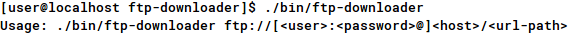
\includegraphics[scale=0.6]{res/usage.png}
    \caption{Utilização do programa}
    \label{fig:usage.png}
\end{figure}

\subsection*{Análise de URL}
Após a leitura e compreensão do \texttt{RFC1738}, desenhou-se uma estrutura de
dados com a finalidade de armazenar a informação extraída da análise de um link
URL recebido pela linha de comandos. Quando fornecidos, são guardados na
estrutura referida, o nome de utilizador, a password, o host, ip, path e nome
do ficheiro em arrays de caracteres independentes. Para além disso, é também
definida a porta 21 como a predefinida na ligação de controlo do protocolo de
FTP. À semelhança do que é referido no \texttt{RFC1738}, caracteres
capitalizados são interpretados como caracteres minúsculos, admitindo ftp da
mesma forma que FTP.

Para se poder resolver o endereço de IP armazenado na estrutura de URL, é feita
uma chamada à função \texttt{gethostbyname} que permite a obtenção do endereço
de uma máquina a partir do nome e retorna uma estrutura do tipo
\texttt{hostent} contendo o endereço na variável \texttt{h\_addr} que é
posteriormente convertido para um array de chars com o auxílio da função
\texttt{inet\_ntoa}.

\subsection*{Cliente de FTP}
O cliente de FTP liga-se através de um socket TCP ao servidor de FTP
identificado pelo endereço de IP acima mencionado e à porta 21 e estabelece uma
ligação de controlo de comunicação, comunicando com uma sequência de comandos
de transferência FTP que lhe são enviados ao estilo do protocolo Telnet: 

\begin{labeling}{alligator}
\item [\textbf{USER user}] envio do nome de utilizador sob a forma de uma string que identifica o utilizador no servidor remoto.
\item [\textbf{PASS pass}] envio da palavra passe completando a identificação no sistema de identificação e controlo de acesso do servidor.
\item [\textbf{CWD path}] indicação do directório que contém o ficheiro requerido para download e sobre o qual se pretende trabalhar.
\item [\textbf{PASV}] comando que pede ao servidor para ficar à escuta numa porta de dados diferente da porta usada pelo serviço de controlo. Este comando recebe uma resposta que contém o endereço e a porta na qual o servidor ficou à escuta para poder estabelecer uma outra ligação TCP usada para transferência de dados.
\item [\textbf{RETR filename}] comando \texttt{retrieve} que pede ao servidor que inicie a transmissão de uma cópia do ficheiro especificado pelo campo \texttt{filename} usando a nova ligação estabelecida ao endereço e porta recebidos pelo comando anterior.
\end{labeling}

Uma vez estabelecida a ligação dedicada de transmissão de dados, estes vão
sendo recebidos de forma ordenada pelo cliente de FTP e armazenados em disco.

\subsection*{Casos de uso}
Um possível caso de uso pode ser o download de um ficheiro de forma anónima do
URL \texttt{ftp://ftp.up.pt/pub/CentOS/filelist.gz}:

\begin{figure}[H]
    \center
    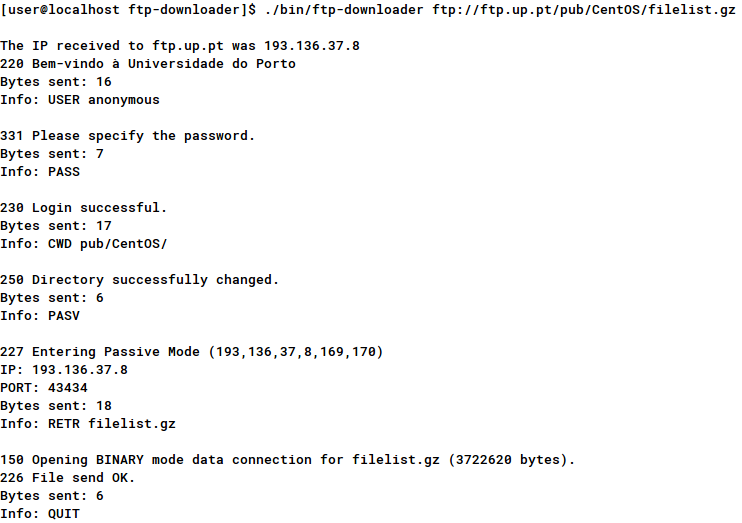
\includegraphics[scale=0.45]{res/anonymous.png}
    \caption{Utilização anónima para download de um ficheiro}
    \label{fig:anonymous.png}
\end{figure}

Também foi testado o download de um ficheiro quando é requerida a autenticação
do utilizador no servidor de FTP:

\begin{figure}[H]
    \center
    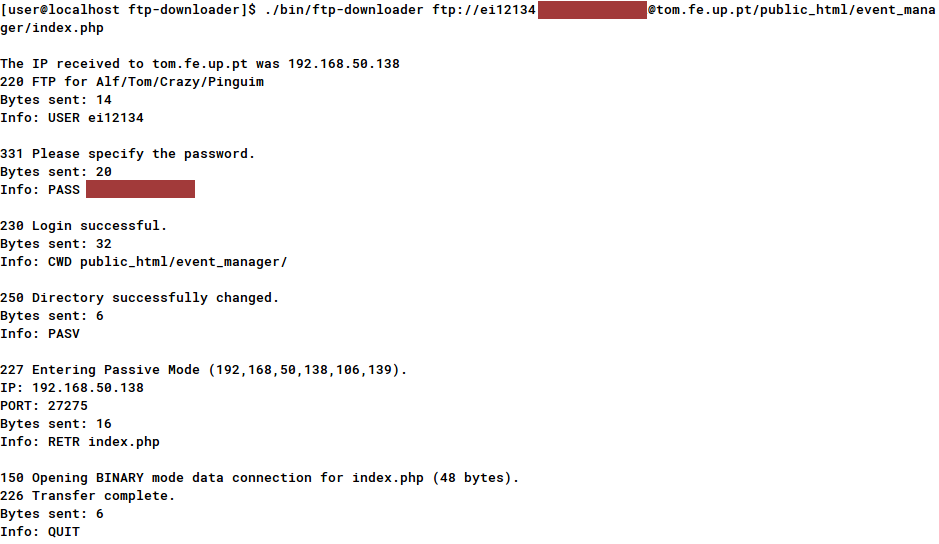
\includegraphics[scale=0.45]{res/authenticated.png}
    \caption{Utilização autenticada no download de um ficheiro}
    \label{fig:authenticated.png}
\end{figure}

\subsection*{Ligações TCP abertas pela aplicação}

\subsection*{Ligação de controlo}

\subsection*{Fases de abertura de uma ligação TCP}

\subsection*{Mecanismo de ARQ em TCP}

\subsection*{Congestionamento na ligação TCP}

\subsection*{Influência de uma segunda ligação TCP}

\section{Experiência 7: Implementação de NAT em Linux }

// TODO

\section{Conclusões}
\iffalse (síntese da informação apresentada nas secções anteriores; reflexão
sobre os objectivos de aprendizagem alcançados) \fi

O projeto pode ser sumariamente descrito pelo seu principal propósito que é o
desenvolvimento de um protocolo de ligação de dados e o seu teste aquando da
obtenção de sucesso na transferência de ficheiros entre dois computadores, com
mecanismos de recuperação face a algumas situações de erros. 


Findo o projeto, consideramos que atingimos os objetivos definidos tendo também
implementado alguns dos elementos de valorização especificados no guião. Esta
abordagem prática permitiu também uma melhor consciência do funcionamento e dos
problemas inerentes às redes comunicações entre computadores, abordados nas
aulas teóricas.

\begin{thebibliography}{9}
\bibitem{lamport93}
  Andrew S. Tanenbaum,
  David J. Wetherall,
  \emph{Computer Networks},
  Prentice Hall, 
  5th edition,
  2011.
\bibitem{rfc1958}
  Network Working Group,
  \emph{Architectural Principles of the Internet},
  June 1996.
\end{thebibliography}

\appendix
\section{Código fonte}
\subsection{Camada de aplicação}
\subsubsection*{netlink.c}
\begin{lstlisting}[style=customcwithlines]
void receiver_stats()
#include <sys/types.h>
#include <sys/stat.h>
#include <fcntl.h>
#include <stdio.h>
#include <string.h>
#include <stdlib.h>
#include <termios.h>
#include <unistd.h>

#include "packets.h"
#include "file.h"
#include "netlink.h"
#include "serial_port.h"

struct file file_to_send;
int max_retries = 3;

void help(char **argv)
{
	fprintf(stderr, "Usage: %s [OPTIONS] <serial port>\n", argv[0]);
	fprintf(stderr, "\n Program options:\n");
	fprintf(stderr, "  -t <FILEPATH>\t\ttransmit file over the serial port\n");
	fprintf(stderr, "  -i\t\t\ttransmit data read from stdin\n");
	fprintf(stderr, "  -b <BAUDRATE>\t\tbaudrate of the serial port\n");
	fprintf(stderr,
			"  -p <DATASIZE>\t\tmaximum bytes of data transfered each frame\n");
	fprintf(stderr, "  -r <RETRY>\t\tnumber of retry attempts\n");
}

int parse_serial_port_arg(int index, char **argv)
{
	if ((strcmp("/dev/ttyS0", argv[index]) != 0)
			&& (strcmp("/dev/ttyS1", argv[index]) != 0)
			&& (strcmp("/dev/ttyS4", argv[index]) != 0)) {
		fprintf(stderr, "Error: bad serial port value\n");
		return -1;
	}

	return index;
}

int parse_baudrate_arg(int baurdate_index, char **argv)
{
	if (strcmp("B50", argv[baurdate_index]) == 0) {
		serial_port_baudrate = B50;
		return 0;
	} else if (strcmp("B75", argv[baurdate_index]) == 0) {
		serial_port_baudrate = B75;
		return 0;
	} else if (strcmp("B110", argv[baurdate_index]) == 0) {
		serial_port_baudrate = B110;
		return 0;
	} else if (strcmp("B134", argv[baurdate_index]) == 0) {
		serial_port_baudrate = B134;
		return 0;
	} else if (strcmp("B150", argv[baurdate_index]) == 0) {
		serial_port_baudrate = B150;
		return 0;
	} else if (strcmp("B200", argv[baurdate_index]) == 0) {
		serial_port_baudrate = B200;
		return 0;
	} else if (strcmp("B300", argv[baurdate_index]) == 0) {
		serial_port_baudrate = B300;
		return 0;
	} else if (strcmp("B600", argv[baurdate_index]) == 0) {
		serial_port_baudrate = B600;
		return 0;
	} else if (strcmp("B1200", argv[baurdate_index]) == 0) {
		serial_port_baudrate = B1200;
		return 0;
	} else if (strcmp("B1800", argv[baurdate_index]) == 0) {
		serial_port_baudrate = B1800;
		return 0;
	} else if (strcmp("B2400", argv[baurdate_index]) == 0) {
		serial_port_baudrate = B2400;
		return 0;
	} else if (strcmp("B4800", argv[baurdate_index]) == 0) {
		serial_port_baudrate = B4800;
		return 0;
	} else if (strcmp("B9600", argv[baurdate_index]) == 0) {
		serial_port_baudrate = B9600;
		return 0;
	} else if (strcmp("B19200", argv[baurdate_index]) == 0) {
		serial_port_baudrate = B19200;
		return 0;
	} else if (strcmp("B38400", argv[baurdate_index]) == 0) {
		serial_port_baudrate = B38400;
		return 0;
	}
	fprintf(stderr, "Error: bad serial port baudrate value\n");
	fprintf(stderr,
			"Valid baudrates: B110, B134, B150, B200, B300, B600, B1200, B1800, B2400, B4800, B9600, B19200, B38400\n");
	return -1;
}

void parse_max_packet_size(int packet_size_index, char **argv)
{
	int val = atoi(argv[packet_size_index]);
	if (val > FRAME_SIZE || val < 0)
		max_data_transfer = FRAME_SIZE;
	else
		max_data_transfer = val;

#ifdef NETLINK_DEBUG_MODE
	fprintf(stderr,"\nparse_max_packet_size:\n");
	fprintf(stderr,"  max_packet_size=%d\n", max_data_transfer);
#endif
}

void parse_max_retries(int packet_size_index, char **argv)
{
	int val = atoi(argv[packet_size_index]);
	if (val <= 0)
		max_retries = 4;
	else
		max_retries = 1 + val;

#ifdef NETLINK_DEBUG_MODE
	fprintf(stderr,"\nmax_retries:\n");
	fprintf(stderr,"  max_retries=%d\n", max_retries);
#endif
}

int parse_flags(int* t_index, int* i_index, int* b_index, int* p_index,
		int* r_index, int argc, char **argv)
{
	for (size_t i = 0; i < (argc - 1); i++) {
		if ((strcmp("-t", argv[i]) == 0)) {
			*t_index = i;
		} else if ((strcmp("-i", argv[i]) == 0)) {
			*i_index = i;
		} else if ((strcmp("-b", argv[i]) == 0)) {
			*b_index = i;
		} else if ((strcmp("-p", argv[i]) == 0)) {
			*p_index = i;
		} else if ((strcmp("-r", argv[i]) == 0)) {
			*r_index = i;
		} else if ((argv[i][0] == '-')) {
			return -1;
		}
	}
#ifdef NETLINK_DEBUG_MODE
	fprintf(stderr,"\nparse_flags(): flag indexes\n");
	fprintf(stderr,"  -t=%d\n  -i=%d\n  -b=%d\n  -p=%d\n  -r=%d\n", *t_index, *i_index, *b_index,
			*p_index, *r_index);
#endif
	return 0;
}

int parse_args(int argc, char **argv, int *is_transmitter)
{

#ifdef NETLINK_DEBUG_MODE
	fprintf(stderr,"\nparse_args(): received arguments\n");
	fprintf(stderr,"  argc=%d\n  argv=%s\n", argc, *argv);
#endif

	if (argc < 2) {
		return -1;
	}

	if (argc == 2)
		return parse_serial_port_arg(1, argv);

	int t_index = -1, i_index = -1, b_index = -1, p_index = -1, r_index = -1;

	if (parse_flags(&t_index, &i_index, &b_index, &p_index, &r_index, argc,
			argv)) {
		fprintf(stderr, "Error: bad flag parameter\n");
		return -1;
	}

	if (t_index > 0 && t_index < argc - 1) {
		if (read_file_from_disk(argv[t_index + 1], &file_to_send) < 0) {
			return -1;
		}
		*is_transmitter = 1;
	} else {
		if (i_index > 0 && i_index < argc - 1) {
			if (read_file_from_stdin(&file_to_send) < 0) {
				return -1;
			}
			*is_transmitter = 1;
		}
	}

	if (b_index > 0 && b_index < argc - 1) {
		if (parse_baudrate_arg(b_index + 1, argv) != 0) {
			return -1;
		}
	}

	if (p_index > 0 && p_index < argc - 1) {
		parse_max_packet_size(p_index + 1, argv);
	}

	if (r_index > 0 && r_index < argc - 1) {
		parse_max_retries(r_index + 1, argv);
	}

	return parse_serial_port_arg(argc - 1, argv);
}

int main(int argc, char **argv)
{
	int port_index = -1;
	int is_transmitter = 0;

	if ((port_index = parse_args(argc, argv, &is_transmitter)) < 0) {
		help(argv);
		exit(EXIT_FAILURE);
	}

	if (is_transmitter) {
		fprintf(stderr, "transmitting %s\n", file_to_send.name);
		return send_file(argv[port_index], &file_to_send, max_retries);
	} else {
		fprintf(stderr, "receiving file\n");
#ifdef NETLINK_DEBUG_MODE
		fprintf(stderr, "\tserial_port_baudrate:%d\n", serial_port_baudrate);
		fprintf(stderr, "\tis_transmitter:%d\n", is_transmitter);
#endif
		return receive_file(argv[port_index], max_retries);
	}
}
\end{lstlisting}


\end{document}

